% Self-contained source for Overleaf.
% Upload this file to the project root, set it as Main document, and use pdfLaTeX.
% Recompile until references settle; inspect the resulting PDF at normal size.
% Target: 3--4 pages. Compilation, pagination, and visual checks remain pending.
% Layout references:
% https://mirrors.ctan.org/macros/latex/contrib/IEEEtran/IEEEtran_HOWTO.pdf
% https://tikz.dev/tikz-shapes
% https://tikz.dev/library-fit
\documentclass[conference]{IEEEtran}

\usepackage[T1]{fontenc}
\usepackage{tikz}
\usepackage{array}
\usepackage{booktabs}
\usepackage[hidelinks]{hyperref}
\usetikzlibrary{positioning,arrows.meta,fit,backgrounds,calc}

% One wide figure per page keeps the two detailed views visually distinct.
\setcounter{dbltopnumber}{1}

\tikzset{
  diagram/.style={font=\sffamily\fontsize{9}{10.5}\selectfont},
  block/.style={
    draw=black!75, fill=black!3, rounded corners=1.2pt,
    line width=0.5pt, align=center, inner sep=3pt,
    minimum height=8mm, text width=18mm
  },
  endpoint/.style={block, fill=white},
  link/.style={
    draw=black!85, line width=0.55pt,
    -{Stealth[length=1.7mm,width=1.2mm]}
  },
  audio/.style={link, line width=0.7pt},
  control/.style={link, dashed},
  power/.style={link, densely dotted, draw=black!65},
  bus/.style={densely dotted, draw=black!65, line width=0.55pt},
  dependency/.style={link},
  tag/.style={
    font=\sffamily\fontsize{8}{9}\selectfont,
    align=center, fill=white, inner sep=0.6pt
  },
  group title/.style={
    font=\sffamily\bfseries\fontsize{9}{10.5}\selectfont,
    align=center, inner sep=1pt
  },
  boundary/.style={
    draw=black!50, line width=0.45pt,
    rounded corners=2pt, inner sep=2.5mm
  }
}

\title{System Architecture of Portable Guitar MultiFX}
\author{
  \IEEEauthorblockN{Javier Estiven Le\'on Calder\'on}
  \IEEEauthorblockA{
    Electronic Engineering\\
    Universidad Nacional de Colombia
  }
}

\begin{document}
\maketitle

\begin{abstract}
Portable Guitar MultiFX is a proposed compact practice amplifier combining
guitar input conditioning, digital effects, simple controls, and loudspeaker
reproduction. Following the architectural views in Chapter~2 of Elecia
White's \emph{Making Embedded Systems}, this report defines the product's
external interactions, decomposes its implementation into functional blocks,
and organizes the proposed controller software by responsibility and
dependency. The architecture separates continuous audio processing from
user-interface control and distinguishes the product enclosure from the
main PCB. Component restrictions are established project constraints;
interfaces, autonomous startup, and complete-system performance still
require verification. These diagrams propose a design, not a validated
prototype.
\end{abstract}

\begin{IEEEkeywords}
Embedded systems, system architecture, guitar effects, DSP, hardware--software
integration.
\end{IEEEkeywords}

\section{Purpose and Architectural Scope}

White's context, block, and organigram views answer different questions:
how the product interacts with its environment, what implements its
functions, and which software responsibilities depend on others~\cite{white}.
The following views retain the same system boundary and functional intent.

The project aims to provide guitar practice with a compact, self-contained
amplifier. Its initial functional target is mono audio with clean and drive
modes, equalization, two buttons, LED feedback, and parameter adjustment
through the DSP module's potentiometers. After programming, normal operation
should require an external power supply but no computer.

The proposed audio platform is a TSA1702B module based on the ADAU1701.
The module documentation describes analog audio interfaces and SigmaStudio
programming~\cite{tsa}; the processor documentation identifies integrated
audio converters, a programmable DSP, and control interfaces~\cite{adau}.
A separate STM32F030C8T6 is proposed for user-interface and DSP-parameter
control. The STM32 family provides GPIO, timing, I\textsuperscript{2}C, and
SWD facilities~\cite{stm}, but their presence does not establish a working
connection to the actual DSP board.

The main PCB is restricted to components from the professor's Altium
library. Other physically obtainable components must connect externally
through headers; use of the DSP module is accepted. Here, \emph{external
to the PCB} can still mean \emph{inside the product}. Amplifier, speaker,
conditioner, connector, and supply selections remain open within those
constraints.

\section{Context: Product and Environment}

Fig.~\ref{fig:context} treats the complete amplifier as a black box. The
guitar supplies an electrical instrument signal. The guitarist selects and
adjusts the sound and receives both acoustic output and visual feedback.
The controls and loudspeaker belong to the product, so they are not
represented as external devices.

\begin{figure}[t]
  \centering
  \begin{tikzpicture}[diagram]
    \node[block,text width=22mm,minimum height=14mm]
      (product) at (0,0) {Portable\\Guitar MultiFX};
    \node[endpoint,text width=12mm]
      (guitar) at (-3.4,0) {Electric\\guitar};
    \node[endpoint,text width=14mm,minimum height=12mm]
      (player) at (3.5,0) {Guitarist};
    \node[endpoint,text width=30mm]
      (supply) at (0,1.95) {External regulated\\power supply};
    \node[endpoint,text width=56mm]
      (tools) at (0,-2.15)
      {Development PC and programmers\\
       DSP: SigmaStudio/USBi \quad MCU: SWD};

    \draw[link] (guitar.east) --
      node[tag,above] {Audio} (product.west);
    \draw[link] (supply.south) --
      node[tag,right] {Power} (product.north);
    \draw[link] ($(player.west)+(0,0.28)$) --
      node[tag,above] {Controls} ($(product.east)+(0,0.28)$);
    \draw[link] ($(product.east)+(0,-0.28)$) --
      node[tag,below,text width=9mm] {Sound\\+ LEDs}
      ($(player.west)+(0,-0.28)$);
    \draw[control,{Stealth[length=1.7mm,width=1.2mm]}-
      {Stealth[length=1.7mm,width=1.2mm]}]
      (tools.north) -- node[tag,right] {Development only} (product.south);
  \end{tikzpicture}
  \caption{Proposed product context. The central box includes the speaker,
  controls, main PCB, and internal modules. The dashed development link
  represents configuration and debugging, not a runtime dependency.}
  \label{fig:context}
\end{figure}

The development equipment configures the DSP and programs or debugs the
controller. USBi and SWD serve different devices and are not interchangeable
programmers. Their depiction describes the intended development workflow,
not confirmed availability of every tool or a verified programming pinout.
The final product must retain the intended DSP program and start without
that equipment.

The supply is intentionally specified by function rather than a fixed
voltage or current. Its final ratings depend on the chosen amplifier,
regulation, actual module inputs, and measured loads. Battery operation,
a display, and additional effects are outside the initial target.

\section{Blocks: Audio, Control, and Power}

Fig.~\ref{fig:blocks} decomposes the product while keeping audio, control,
and power distinct. The conditioner provides an appropriate load for guitar
pickups and adapts the signal to the module input. Its gain, bias, protection,
and usable input range must be selected together; a connector alone does
not provide this adaptation.

\begin{figure*}[t]
  \centering
  \begin{tikzpicture}[diagram]
    % Audio row: coordinates in centimetres; no whole-figure scaling.
    \node[endpoint,text width=11mm]
      (guitar) at (-2.55,0) {Electric\\guitar};
    \node[block] (input) at (0.25,0) {High-Z\\conditioner};
    \node[block,text width=10mm] (adc) at (2.75,0) {ADC};
    \node[block] (dsp) at (5.25,0) {ADAU1701\\Clean / drive\\EQ / level};
    \node[block,text width=10mm] (dac) at (7.75,0) {DAC};
    \node[block] (amp) at (10.4,0) {Power\\amplifier};
    \node[block,text width=14mm]
      (speaker) at (12.8,0) {Speaker};
    \node[block,text width=26mm]
      (pots) at (5.25,-1.45) {Module\\potentiometers};
    \node[group title] (module-title) at (5.25,1.0)
      {TSA1702B module};

    % Main PCB: control, user interface, and supply distribution.
    \node[block,minimum height=12mm]
      (distribution) at (0.25,-4.15) {Power\\distribution\\Rails TBD};
    \node[block] (buttons) at (3.4,-4.15) {Two\\buttons};
    \node[block,text width=28mm,minimum height=12mm]
      (mcu) at (6.8,-4.15) {STM32F030C8T6\\UI / DSP control\\Proposed};
    \node[block] (leds) at (10.65,-4.15) {LED\\indicators};
    \node[group title] (pcb-title) at (5.3,-3.1) {Main PCB};
    \node[endpoint,text width=11mm]
      (power-input) at (-2.55,-4.15) {Power\\input};
    \coordinate (rail-top-left) at (-0.95,2.1);
    \coordinate (rail-top-right) at (10.4,2.1);
    \coordinate (rail-low) at (6.8,-5.4);

    % Draw the largest enclosure first, behind all functional blocks.
    \begin{scope}[on background layer]
      \node[boundary,inner sep=4mm,fill=white,
        fit=(input)(adc)(dac)(dsp)(pots)(module-title)(amp)(speaker)
            (distribution)(buttons)(mcu)(leds)(pcb-title)
            (rail-top-left)(rail-top-right)(rail-low),
        label={[group title,anchor=south west]north west:
          Complete MultiFX product (proposed)}] (product) {};
      \node[boundary,fill=black!2,
        fit=(adc)(dsp)(dac)(pots)(module-title)] (module) {};
      \node[boundary,fill=black!2,
        fit=(distribution)(buttons)(mcu)(leds)(pcb-title)(rail-low)]
        (pcb) {};
    \end{scope}

    \draw[audio] (guitar.east) --
      node[tag,above] {Inst.} (input.west);
    \draw[audio] (input.east) --
      node[tag,above] {Line} (adc.west);
    \draw[audio] (adc.east) --
      node[tag,above] {PCM} (dsp.west);
    \draw[audio] (dsp.east) --
      node[tag,above] {PCM} (dac.west);
    \draw[audio] (dac.east) --
      node[tag,above] {Line} (amp.west);
    \draw[audio] (amp.east) -- (speaker.west);

    \draw[control] (pots.north) -- (dsp.south);
    \draw[control] (buttons.east) --
      node[tag,above] {GPIO} (mcu.west);
    \draw[control] (mcu.east) --
      node[tag,above] {GPIO} (leds.west);
    % Reach a separate control port without crossing the potentiometers
    % or joining the DSP-to-DAC audio connection.
    \draw[control,{Stealth[length=1.7mm,width=1.2mm]}-
      {Stealth[length=1.7mm,width=1.2mm]}]
      (mcu.north) -- (6.8,-2.6) -- (8.9,-2.6) --
      (8.9,-0.85) -- (6.55,-0.85) -- (dsp.south east);
    \node[tag,anchor=west,text width=33mm] at (9.05,-1.7)
      {I\textsuperscript{2}C control\\Interface unverified};

    % A functional distribution bus, not an electrical net or common rail.
    \draw[power] (power-input.east) --
      node[tag,above] {DC} (distribution.west);
    \draw[bus] (distribution.north) -- (0.25,-2.7) --
      (-0.95,-2.7) -- (rail-top-left) -- (rail-top-right);
    \draw[power] (0.25,2.1) -- (input.north);
    \draw[power] (5.25,2.1) -- (module.north);
    \draw[power] (10.4,2.1) -- (amp.north);
    \draw[power] (distribution.south) -- (0.25,-5.4) --
      node[tag,above] {MCU rail} (rail-low) -- (mcu.south);
    \node[tag] at (5.25,2.32) {Distribution rails: ratings TBD};

    \draw[audio] (0,-6.3) -- (0.8,-6.3)
      node[tag,right] {Audio};
    \draw[control] (3.3,-6.3) -- (4.1,-6.3)
      node[tag,right] {Control};
    \draw[power] (7.0,-6.3) -- (7.8,-6.3)
      node[tag,right] {Power distribution};
  \end{tikzpicture}
  \caption{Proposed functional implementation. ADC, DSP, and DAC are logical
  functions of the ADAU1701, not three additional ICs. The speaker and
  external modules remain inside the product; links crossing the main-PCB
  boundary require defined headers. Dotted routes denote supply
  distribution and may represent different regulated rails, not one
  electrically common net. Audio after the amplifier drives the speaker.}
  \label{fig:blocks}
\end{figure*}

The ADC, DSP, and DAC functions belong to the ADAU1701~\cite{adau}.
The proposed SigmaStudio program supplies clean routing, drive, EQ, level
management, and smooth parameter changes. These functions and the
potentiometer assignments must be implemented and checked in the actual
program. The module's analog output is a signal-level interface to a
separate amplifier; the power stage, rather than the DSP output, drives
the loudspeaker.

The STM32 handles buttons, indicators, and control transactions. It does
not transport audio samples. The module potentiometers act on DSP
parameters directly through the module's control facilities. Their mapping
is independent of the controller's button sampling.

An I\textsuperscript{2}C link is proposed, but its access on the actual
TSA1702B, logic levels, addressing, and interaction with USBi remain
unverified. The ADAU1701 supports EEPROM self-boot~\cite{adau}; controller
transactions must respect that sequence. Runtime control must use the
parameter addresses and formats exported for the matching SigmaStudio
program.

The dotted supply routes express responsibility for powering each active
subsystem. They are not a wiring schematic: a common distribution source
does not imply identical voltages at all loads. Connector ratings,
regulation, returns, decoupling, and transient demand require a separate
electrical design.

\section{Organigram: Software Responsibilities}

Fig.~\ref{fig:organigram} applies White's organigram as a hierarchy of
software responsibilities and dependencies~\cite{white}. It is a proposed
organization of the controller software, not an execution sequence or an
organization of people.

\begin{figure*}[t]
  \centering
  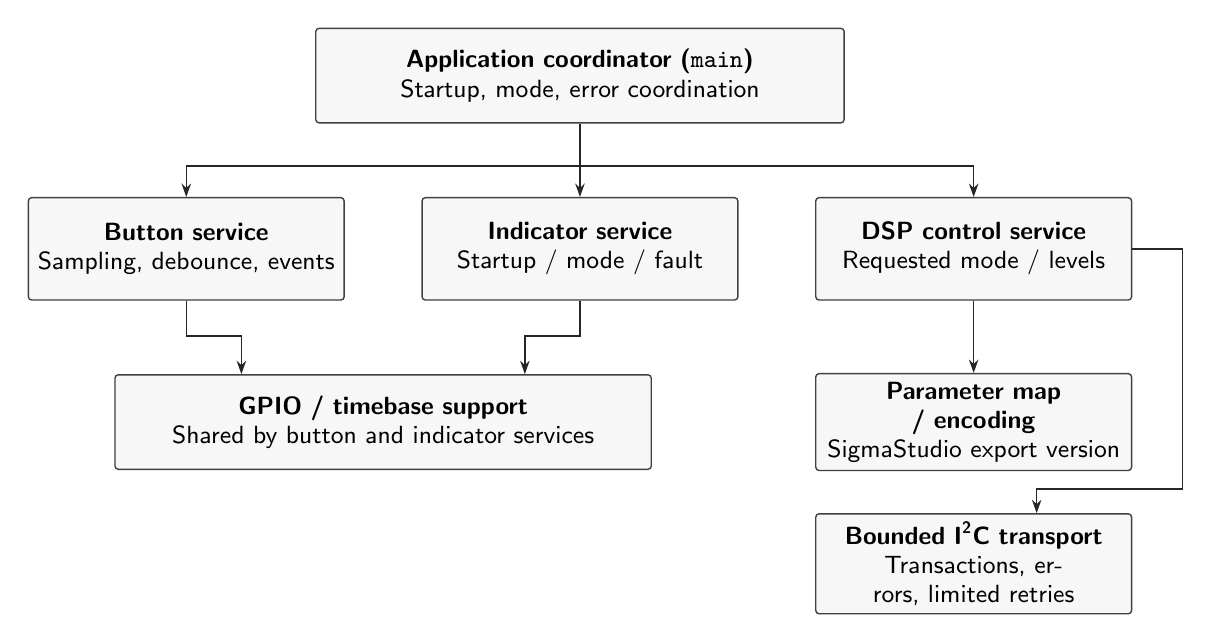
\begin{tikzpicture}[diagram]
    \node[block,text width=65mm,minimum height=12mm]
      (application) at (0,0)
      {\textbf{Application coordinator (\texttt{main})}\\
       Startup, mode, error coordination};
    \node[block,text width=38mm,minimum height=13mm]
      (buttons) at (-5,-2.2)
      {\textbf{Button service}\\Sampling, debounce, events};
    \node[block,text width=38mm,minimum height=13mm]
      (indicators) at (0,-2.2)
      {\textbf{Indicator service}\\Startup / mode / fault};
    \node[block,text width=38mm,minimum height=13mm]
      (dsp-control) at (5,-2.2)
      {\textbf{DSP control service}\\Requested mode / levels};
    \node[block,text width=66mm,minimum height=12mm]
      (gpio) at (-2.5,-4.4)
      {\textbf{GPIO / timebase support}\\
       Shared by button and indicator services};
    \node[block,text width=38mm,minimum height=12mm]
      (parameters) at (5,-4.4)
      {\textbf{Parameter map / encoding}\\SigmaStudio export version};
    \node[block,text width=38mm,minimum height=12mm]
      (transport) at (5,-6.2)
      {\textbf{Bounded I\textsuperscript{2}C transport}\\
       Transactions, errors, limited retries};

    \coordinate (dispatch) at (0,-1.15);
    \draw[draw=black!85,line width=0.55pt]
      (application.south) -- (dispatch);
    \draw[dependency] (dispatch) -| (buttons.north);
    \draw[dependency] (dispatch) -- (indicators.north);
    \draw[dependency] (dispatch) -| (dsp-control.north);
    \draw[dependency] (buttons.south) -- ++(0,-0.45) -|
      ($(gpio.north)+(-18mm,0)$);
    \draw[dependency] (indicators.south) -- ++(0,-0.45) -|
      ($(gpio.north)+(18mm,0)$);
    \draw[dependency] (dsp-control.south) -- (parameters.north);
    % Mapping/encoding and transport are separate service dependencies.
    \draw[dependency] (dsp-control.east) -- (7.65,-2.2) --
      (7.65,-5.25) -| ($(transport.north)+(8mm,0)$);
  \end{tikzpicture}
  \caption{Proposed controller-software organigram. Downward arrows denote
  dependencies, not audio flow or temporal order. Lower services return
  events, status, and errors to their callers. The shared GPIO/timebase
  block exposes a common platform dependency; the separately deployed
  SigmaStudio audio program is outside this hierarchy.}
  \label{fig:organigram}
\end{figure*}

The application coordinator establishes startup order, maintains the
operating mode, requests parameter changes, and determines the visible
response to communication errors. Button handling produces debounced
events; indicator handling converts application state into LED patterns.
Both depend on board-specific GPIO and timing support. Sharing that support
does not authorize competing ownership of the same output pin.

The DSP control service separates the requested musical behavior from
device-specific parameter representations. A matching export defines
addresses and numerical encoding; the transport supplies bounded
transactions and explicit errors. GPIO, timing, and transport initialization
belong to board support, with startup coordinated by the application.
This view identifies responsibilities without fixing a framework, RTOS,
file-per-box implementation, or final scheduling method.

The hierarchy also defines an error contract: a transport error returns to
the application through the DSP service. The controller can indicate a
persistent fault and suspend parameter changes. It cannot guarantee a mute
or a return to clean through a failed control link. Such behavior would
require a separately defined and verified mechanism.

\section{Consistency and Validation}

The three views describe one product: external interactions in
Fig.~\ref{fig:context}, functional implementation in Fig.~\ref{fig:blocks},
and controller-software dependencies in Fig.~\ref{fig:organigram}. The DSP
audio program and MCU firmware are separate deployments linked by a
versioned parameter contract. The main PCB integrates permitted components
and module interfaces; it does not duplicate the entire commercial DSP
board.

\begin{table}[t]
  \caption{Interface Requirements Still to Verify}
  \label{tab:interfaces}
  \centering
  \footnotesize
  \setlength{\tabcolsep}{3pt}
  \renewcommand{\arraystretch}{1.12}
  \begin{tabular}{@{}>{\raggedright\arraybackslash}p{0.24\columnwidth}
                      >{\raggedright\arraybackslash}p{0.69\columnwidth}@{}}
    \toprule
    Interface & Required evidence before design release \\
    \midrule
    Guitar to ADC &
      Actual input impedance, bias, gain, accepted signal range,
      and unclipped operation with the conditioner. \\
    DSP to amplifier &
      Compatible output level, input sensitivity, gain, speaker load,
      and measured clean output. \\
    External DSP control &
      Accessible bus, logic levels, addressing, parameter format/version,
      and successful commands on the actual board. \\
    Power and startup &
      Correct rails, load/transient budget, repeatable autonomous boot,
      and coordination of DSP, MCU, and programmer access. \\
    \bottomrule
  \end{tabular}
\end{table}

Table~\ref{tab:interfaces} defines verification work rather than reporting
results. The module and USBi are reported available; no complete audio-chain
test, deployed controller firmware, fabricated MultiFX PCB, or validated
system power budget is recorded. Manufacturer capabilities are design
inputs, not measured prototype specifications.

Before committing to the PCB, identify the actual board and native library,
demonstrate clean audio, verify autonomous startup without a computer, and
measure the effect of an externally commanded DSP parameter change.
Record hardware identity, software/export versions, connections, signal
conditions, expected behavior, and observed results. These tests reduce the
critical integration risks while retaining the component boundary and
keeping unproven performance claims out of the design.

\begin{thebibliography}{4}

\bibitem{white}
E.~White, \emph{Making Embedded Systems: Design Patterns for Great
Software}, 2nd~ed. O'Reilly Media, 2024, ch.~2.

\bibitem{tsa}
TinySine, \textquotedblleft{}TSA1702B: Bluetooth 5.1 + DSP Audio Receiver
Board,\textquotedblright{} datasheet. Accessed: Oct.~20, 2026.
[Online]. Available:
\url{https://www.tinyosshop.com/datasheet/TSA1702B_Datasheet.pdf}

\bibitem{adau}
Analog Devices, \textquotedblleft{}ADAU1701: SigmaDSP 28-/56-bit audio
processor with two ADCs and four DACs,\textquotedblright{} datasheet,
rev.~C, 2016. [Online]. Available:
\url{https://www.analog.com/media/en/technical-documentation/data-sheets/ADAU1701.pdf}

\bibitem{stm}
STMicroelectronics, \textquotedblleft{}STM32F030x4/x6/x8/xC,\textquotedblright{}
datasheet DS9773, rev.~5, Nov.~2021. [Online]. Available:
\url{https://www.st.com/resource/en/datasheet/stm32f030c8.pdf}

\end{thebibliography}
\end{document}
